
%% bare_conf.tex
%% V1.4b
%% 2015/08/26
%% by Michael Shell
%% See:
%% http://www.michaelshell.org/
%% for current contact information.
%%
%% This is a skeleton file demonstrating the use of IEEEtran.cls
%% (requires IEEEtran.cls version 1.8b or later) with an IEEE
%% conference paper.
%%
%% Support sites:
%% http://www.michaelshell.org/tex/ieeetran/
%% http://www.ctan.org/pkg/ieeetran
%% and
%% http://www.ieee.org/

%%*************************************************************************
%% Legal Notice:
%% This code is offered as-is without any warranty either expressed or
%% implied; without even the implied warranty of MERCHANTABILITY or
%% FITNESS FOR A PARTICULAR PURPOSE! 
%% User assumes all risk.
%% In no event shall the IEEE or any contributor to this code be liable for
%% any damages or losses, including, but not limited to, incidental,
%% consequential, or any other damages, resulting from the use or misuse
%% of any information contained here.
%%
%% All comments are the opinions of their respective authors and are not
%% necessarily endorsed by the IEEE.
%%
%% This work is distributed under the LaTeX Project Public License (LPPL)
%% ( http://www.latex-project.org/ ) version 1.3, and may be freely used,
%% distributed and modified. A copy of the LPPL, version 1.3, is included
%% in the base LaTeX documentation of all distributions of LaTeX released
%% 2003/12/01 or later.
%% Retain all contribution notices and credits.
%% ** Modified files should be clearly indicated as such, including  **
%% ** renaming them and changing author support contact information. **
%%*************************************************************************


% *** Authors should verify (and, if needed, correct) their LaTeX system  ***
% *** with the testflow diagnostic prior to trusting their LaTeX platform ***
% *** with production work. The IEEE's font choices and paper sizes can   ***
% *** trigger bugs that do not appear when using other class files.       ***                          ***
% The testflow support page is at:
% http://www.michaelshell.org/tex/testflow/



\documentclass[conference]{IEEEtran}
% Some Computer Society conferences also require the compsoc mode option,
% but others use the standard conference format.
%
% If IEEEtran.cls has not been installed into the LaTeX system files,
% manually specify the path to it like:
% \documentclass[conference]{../sty/IEEEtran}





% Some very useful LaTeX packages include:
% (uncomment the ones you want to load)


% *** MISC UTILITY PACKAGES ***
%
%\usepackage{ifpdf}
% Heiko Oberdiek's ifpdf.sty is very useful if you need conditional
% compilation based on whether the output is pdf or dvi.
% usage:
% \ifpdf
%   % pdf code
% \else
%   % dvi code
% \fi
% The latest version of ifpdf.sty can be obtained from:
% http://www.ctan.org/pkg/ifpdf
% Also, note that IEEEtran.cls V1.7 and later provides a builtin
% \ifCLASSINFOpdf conditional that works the same way.
% When switching from latex to pdflatex and vice-versa, the compiler may
% have to be run twice to clear warning/error messages.






% *** CITATION PACKAGES ***
%
%\usepackage{cite}
% cite.sty was written by Donald Arseneau
% V1.6 and later of IEEEtran pre-defines the format of the cite.sty package
% \cite{} output to follow that of the IEEE. Loading the cite package will
% result in citation numbers being automatically sorted and properly
% "compressed/ranged". e.g., [1], [9], [2], [7], [5], [6] without using
% cite.sty will become [1], [2], [5]--[7], [9] using cite.sty. cite.sty's
% \cite will automatically add leading space, if needed. Use cite.sty's
% noadjust option (cite.sty V3.8 and later) if you want to turn this off
% such as if a citation ever needs to be enclosed in parenthesis.
% cite.sty is already installed on most LaTeX systems. Be sure and use
% version 5.0 (2009-03-20) and later if using hyperref.sty.
% The latest version can be obtained at:
% http://www.ctan.org/pkg/cite
% The documentation is contained in the cite.sty file itself.






% *** GRAPHICS RELATED PACKAGES ***
%
\ifCLASSINFOpdf
\usepackage{placeins}
  \usepackage[pdftex]{graphicx}
  % declare the path(s) where your graphic files are
   \graphicspath{}
  % and their extensions so you won't have to specify these with
  % every instance of \includegraphics
  % \DeclareGraphicsExtensions{.pdf,.jpeg,.png}
\else
  % or other class option (dvipsone, dvipdf, if not using dvips). graphicx
  % will default to the driver specified in the system graphics.cfg if no
  % driver is specified.
  % \usepackage[dvips]{graphicx}
  % declare the path(s) where your graphic files are
  % \graphicspath{{../eps/}}
  % and their extensions so you won't have to specify these with
  % every instance of \includegraphics
  % \DeclareGraphicsExtensions{.eps}
\fi
% graphicx was written by David Carlisle and Sebastian Rahtz. It is
% required if you want graphics, photos, etc. graphicx.sty is already
% installed on most LaTeX systems. The latest version and documentation
% can be obtained at: 
% http://www.ctan.org/pkg/graphicx
% Another good source of documentation is "Using Imported Graphics in
% LaTeX2e" by Keith Reckdahl which can be found at:
% http://www.ctan.org/pkg/epslatex
%
% latex, and pdflatex in dvi mode, support graphics in encapsulated
% postscript (.eps) format. pdflatex in pdf mode supports graphics
% in .pdf, .jpeg, .png and .mps (metapost) formats. Users should ensure
% that all non-photo figures use a vector format (.eps, .pdf, .mps) and
% not a bitmapped formats (.jpeg, .png). The IEEE frowns on bitmapped formats
% which can result in "jaggedy"/blurry rendering of lines and letters as
% well as large increases in file sizes.
%
% You can find documentation about the pdfTeX application at:
% http://www.tug.org/applications/pdftex





% *** MATH PACKAGES ***
%
%\usepackage{amsmath}
% A popular package from the American Mathematical Society that provides
% many useful and powerful commands for dealing with mathematics.
%
% Note that the amsmath package sets \interdisplaylinepenalty to 10000
% thus preventing page breaks from occurring within multiline equations. Use:
%\interdisplaylinepenalty=2500
% after loading amsmath to restore such page breaks as IEEEtran.cls normally
% does. amsmath.sty is already installed on most LaTeX systems. The latest
% version and documentation can be obtained at:
% http://www.ctan.org/pkg/amsmath





% *** SPECIALIZED LIST PACKAGES ***
%
%\usepackage{algorithmic}
% algorithmic.sty was written by Peter Williams and Rogerio Brito.
% This package provides an algorithmic environment fo describing algorithms.
% You can use the algorithmic environment in-text or within a figure
% environment to provide for a floating algorithm. Do NOT use the algorithm
% floating environment provided by algorithm.sty (by the same authors) or
% algorithm2e.sty (by Christophe Fiorio) as the IEEE does not use dedicated
% algorithm float types and packages that provide these will not provide
% correct IEEE style captions. The latest version and documentation of
% algorithmic.sty can be obtained at:
% http://www.ctan.org/pkg/algorithms
% Also of interest may be the (relatively newer and more customizable)
% algorithmicx.sty package by Szasz Janos:
% http://www.ctan.org/pkg/algorithmicx




% *** ALIGNMENT PACKAGES ***
%
%\usepackage{array}
% Frank Mittelbach's and David Carlisle's array.sty patches and improves
% the standard LaTeX2e array and tabular environments to provide better
% appearance and additional user controls. As the default LaTeX2e table
% generation code is lacking to the point of almost being broken with
% respect to the quality of the end results, all users are strongly
% advised to use an enhanced (at the very least that provided by array.sty)
% set of table tools. array.sty is already installed on most systems. The
% latest version and documentation can be obtained at:
% http://www.ctan.org/pkg/array


% IEEEtran contains the IEEEeqnarray family of commands that can be used to
% generate multiline equations as well as matrices, tables, etc., of high
% quality.




% *** SUBFIGURE PACKAGES ***
%\ifCLASSOPTIONcompsoc
%  \usepackage[caption=false,font=normalsize,labelfont=sf,textfont=sf]{subfig}
%\else
%  \usepackage[caption=false,PACKAGES ***
%font=footnotesize]{subfig}
%\fi
% subfig.sty, written by Steven Douglas Cochran, is the modern replacement
% for subfigure.sty, the latter of which is no longer maintained and is
% incompatible with some LaTeX packages including fixltx2e. However,
% subfig.sty requires and automatically loads Axel Sommerfeldt's caption.sty
% which will override IEEEtran.cls' handling of captions and this will result
% in non-IEEE style figure/table captions. To prevent this problem, be sure
% and invoke subfig.sty's "caption=false" package option (available since
% subfig.sty version 1.3, 2005/06/28) as this is will preserve IEEEtran.cls
% handling of captions.
% Note that the Computer Society format requires a larger sans serif font
% than the serif footnote size font used in traditional IEEE formatting
% and thus the need to invoke different subfig.sty package options depending
% on whether compsoc mode has been enabled.
%
% The latest version and documentation of subfig.sty can be obtained at:
% http://www.ctan.org/pkg/subfig




% *** FLOAT PACKAGES ***
%
%\usepackage{fixltx2e}
% fixltx2e, the successor to the earlier fix2col.sty, was written by
% Frank Mittelbach and David Carlisle. This package corrects a few problems
% in the LaTeX2e kernel, the most notable of which is that in current
% LaTeX2e releases, the ordering of single and double column floats is not
% guaranteed to be preserved. Thus, an unpatched LaTeX2e can allow a
% single column figure to be placed prior to an earlier double column
% figure.
% Be aware that LaTeX2e kernels dated 2015 and later have fixltx2e.sty's
% corrections already built into the system in which case a warning will
% be issued if an attempt is made to load fixltx2e.sty as it is no longer
% needed.
% The latest version and documentation can be found at:
% http://www.ctan.org/pkg/fixltx2e


%\usepackage{stfloats}
% stfloats.sty was written by Sigitas Tolusis. This package gives LaTeX2e
% the ability to do double column floats at the bottom of the page as well
% as the top. (e.g., "\begin{figure*}[!b]" is not normally possible in
% LaTeX2e). It also provides a command:
%\fnbelowfloat
% to enable the placement of footnotes below bottom floats (the standard
% LaTeX2e kernel puts them above bottom floats). This is an invasive package
% which rewrites many portions of the LaTeX2e float routines. It may not work
% with other packages that modify the LaTeX2e float routines. The latest
% version and documentation can be obtained at:
% http://www.ctan.org/pkg/stfloats
% Do not use the stfloats baselinefloat ability as the IEEE does not allow
% \baselineskip to stretch. Authors submitting work to the IEEE should note
% that the IEEE rarely uses double column equations and that authors should try
% to avoid such use. Do not be tempted to use the cuted.sty or midfloat.sty
% packages (also by Sigitas Tolusis) as the IEEE does not format its papers in
% such ways.
% Do not attempt to use stfloats with fixltx2e as they are incompatible.
% Instead, use Morten Hogholm'a dblfloatfix which combines the features
% of both fixltx2e and stfloats:
%
% \usepackage{dblfloatfix}
% The latest version can be found at:
% http://www.ctan.org/pkg/dblfloatfix




% *** PDF, URL AND HYPERLINK PACKAGES ***
%
%\usepackage{url}
% url.sty was written by Donald Arseneau. It provides better support for
% handling and breaking URLs. url.sty is already installed on most LaTeX
% systems. The latest version and documentation can be obtained at:
% http://www.ctan.org/pkg/url
% Basically, \url{my_url_here}.




% *** Do not adjust lengths that control margins, column widths, etc. ***
% *** Do not use packages that alter fonts (such as pslatex).         ***
% There should be no need to do such things with IEEEtran.cls V1.6 and later.
% (Unless specifically asked to do so by the journal or conference you plan
% to submit to, of course. )


% correct bad hyphenation here
\hyphenation{op-tical net-works semi-conduc-tor}


\begin{document}
%
% paper title
% Titles are generally capitalized except for words such as a, an, and, as,
% at, but, by, for, in, nor, of, on, or, the, to and up, which are usually
% not capitalized unless they are the first or last word of the title.
% Linebreaks \\ can be used within to get better formatting as desired.
% Do not put math or special symbols in the title.
\title{Fast Switched-Capacitor Moving Average Filter for Direct Sampling Mixers}


% author names and affiliations
% use a multiple column layout for up to three different
% affiliations
\author{\IEEEauthorblockN{Cole A. Nielsen}
\IEEEauthorblockA{Electrical and Computer Engineering\\
University of Minnesota - Twin Cities\\
Minneapolis, MN 55455\\
niels538@umn.edu}
}
% conference papers do not typically use \thanks and this command
% is locked out in conference mode. If really needed, such as for
% the acknowledgment of grants, issue a \IEEEoverridecommandlockouts
% after \documentclass

% for over three affiliations, or if they all won't fit within the width
% of the page, use this alternative format:
% 
%\author{\IEEEauthorblockN{Michael Shell\IEEEauthorrefmark{1},
%Homer Simpson\IEEEauthorrefmark{2},
%James Kirk\IEEEauthorrefmark{3}, 
%Montgomery Scott\IEEEauthorrefmark{3} and
%Eldon Tyrell\IEEEauthorrefmark{4}}
%\IEEEauthorblockA{\IEEEauthorrefmark{1}School of Electrical and Computer Engineering\\
%Georgia Institute of Technology,
%Atlanta, Georgia 30332--0250\\ Email: see http://www.michaelshell.org/contact.html}
%\IEEEauthorblockA{\IEEEauthorrefmark{2}Twentieth Century Fox, Springfield, USA\\
%Email: homer@thesimpsons.com}
%\IEEEauthorblockA{\IEEEauthorrefmark{3}Starfleet Academy, San Francisco, California 96678-2391\\
%Telephone: (800) 555--1212, Fax: (888) 555--1212}
%\IEEEauthorblockA{\IEEEauthorrefmark{4}Tyrell Inc., 123 Replicant Street, Los Angeles, California 90210--4321}}




% use for special paper notices
%\IEEEspecialpapernotice{(Invited Paper)}




% make the title area
\maketitle

% As a general rule, do not put math, special symbols or citations
% in the abstract
\begin{abstract}
A moving average filter design utilizing a switched capacitor circuit is described. The moving average filter was implemented with a high gain and high-speed telescopic op amp with minimum channel lengths in the FreePDK45 process. The final design is able to drive up to 1pF of load to a gain bandwidth of 731 MHz with a phase margin of 89 degrees, making it very stable. The switched capacitor circuit failed to work as designed due to deficiencies with the common mode feedback of the OP amp design decgrading performance.
\end{abstract}

% no keywords




% For peer review papers, you can put extra information on the cover
% page as needed:
% \ifCLASSOPTIONpeerreview
% \begin{center} \bfseries EDICS Category: 3-BBND \end{center}
% \fi
%
% For peerreview papers, this IEEEtran command inserts a page break and
% creates the second title. It will be ignored for other modes.
\IEEEpeerreviewmaketitle



\section{Introduction}
% no \IEEEPARstart
Recent industrial trends push for the continual reduction in size as well as power consumption of consumer electronic devices, essentially all of which contain some form of a wireless radio. At the core of these radios are mixers, used to upconvert and downconvert signals between frequencies. Conventional receiver architectures rely on one heterodyne receiver per band, which consumes large amounts of area and power for multi band systems. Direct sampled mixer approaches (e.g. MTDSM) offer a huge advantage where one mixer circuit can be used across a wide band (covering many bands), reducing die area and power usage simple by decreasing the number of circuits needed \cite{IEEEhowto:new}.\par
 
In lieu of the advantages of direct sampled mixers and their future prospect, a switched capacitor moving average filter was designed in for this project for application to direct sampling mixers. More specifically, a high performance telescopic op amp was designed as well as a switched capacitor network.

\section{Design Architecture}
A prototypical direct sampled mixer utilizing a switched capacitor is shown in figure \ref{a} \cite{IEEEhowto:ninh}. This circuit is the basis of this design project. This circuit features a LNTA, a mixer, and a SC moving average filter. As the mixer and LNTA designs are a different subject matter than that taught in 5333, only the SC part of the design was considered in this project. More specifically only the first stage of the SC cicuit was designed to avoid over complication the project.\par
A brief overview of the operation of the moving average filter is as follows: a current coming out of the RF section of the design is fed into the sampling portion of the circuit (at the caps labeled Cs). The input current contains the mixed RF signal to be filtered. The input of the MA filter then uses four switched sampling capacitors (2 per input) to convert the input current to charge (sampling in this system works on charge), with each input having two samplers that alternate sampling twice a period to yield a continuous output signal (no gaps in the sampling). The charge of Cs is then shared with a history capacitor (Ch), larger then CS, on the time Cs is not being used to sample. This sharing of charge acts as a means of implementing a IIR filter, in this case a moving average filter. The output of the circuit is then shared onto an output cap Co for measing by an ADC. The output of the circuit ideally should smooth out an input signal, isolating a downconverted signal from higher harmonics if a mixed signal is fed into the circuit.\par
The architecture of the opamp was chosen to be high bandwidth and high speed. This is to ensure high speed filtering of input signals, as well as ensuring fast settling times. To meet these needs, a telescopic op amp design with gain boosting and common mode feedback was selected.Initially a folded cascode was selected for this project, however this was changed as the benefits in terms of gain, bandwidth, and power consumption of a telescopic topology was realized (specifically the 2x lower current consumption).
\begin{figure}
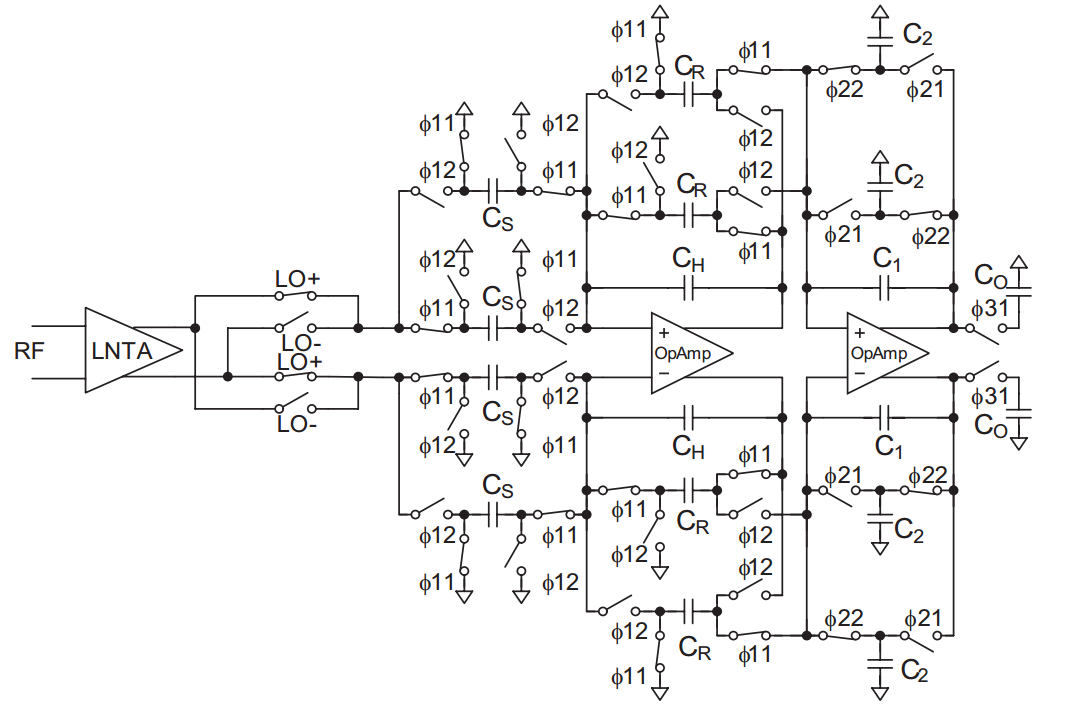
\includegraphics[width=0.5\textwidth]{cir.png}
\caption{Direct Sampling Mixer Architecture \cite{IEEEhowto:ninh}}
\label{a}
\end{figure}
\section*{Operational Amplifier Design}
Below is a table summarizing the performance of the designed telescopic op amp.

\begin{figure}[htb]
\centering
\begin{tabular}[width=\textwidth]{|c|c|}
\hline \rule[-2ex]{0pt}{5.5ex} \textbf{Parameter} & \textbf{Measured (target)}  \\ 
\hline \rule[-2ex]{0pt}{5.5ex} Voltage Gain & 56dB (100db) \\ 
\hline \rule[-2ex]{0pt}{5.5ex} Unity Gain Bandwidth & 731 MHz (1GHz)\\ 
\hline \rule[-2ex]{0pt}{5.5ex} Slew Rate & 500 V/$\mu$s (750 V/$\mu$s) \\ 
\hline \rule[-2ex]{0pt}{5.5ex} Temperature Range & 0-$70^\circ$C  \\ 
\hline \rule[-2ex]{0pt}{5.5ex} Load Capacitance & 1pF \\ 
\hline \rule[-2ex]{0pt}{5.5ex} Phase Margin & $89^\circ$ ($60^\circ$) \\ 
\hline \rule[-2ex]{0pt}{5.5ex} Supply Voltage &  $1.25$V\\ 
\hline \rule[-2ex]{0pt}{5.5ex} Input Common Mode Voltage & 0.55 - 0.9v \\ 
\hline \rule[-2ex]{0pt}{5.5ex} Output Common Mode Voltage &  0.3 - 1.05V\\ 
\hline \rule[-2ex]{0pt}{5.5ex} Power &  1650$\mu$W/1.31mA (1000$\mu$W)\\ 
\hline \rule[-2ex]{0pt}{5.5ex} FOM &  0.558 GHz pF/mA\\ 
\hline 
\end{tabular} 
\caption{OP amp Specifications}
\label{lnta}
\end{figure}
Some of the design specs were low, due to initially too aggressive targets.\par

The full design implemented is shown in the following figure. The circuit is a telescopic cascode with gain boosting and input common mode feedback. The starting point for this design was the gain bandwidth, load capacitance. From these numbers and the FOM for the project, 1mA bias current for the cascode was decided upon. From there, 0.1V Vds was chosen to allow for large output swing. Running several simulations sweeping the size of the cascode transistors showed 10u to be the optimal size for having the input common level be half Vdd. From there I sized the tail mosfet to twice the cascode ones, and the PFETS to also be 2x to lower the VGS. This design also has gain boosing, shown as the triangles, implemented as two stage op amps that take in a reference which sets the quiescent point to the node between the cascode transistors. There is also a CM input FB circuit. These will be discussed next.

\FloatBarrier
\begin{figure}[htb]
\centering
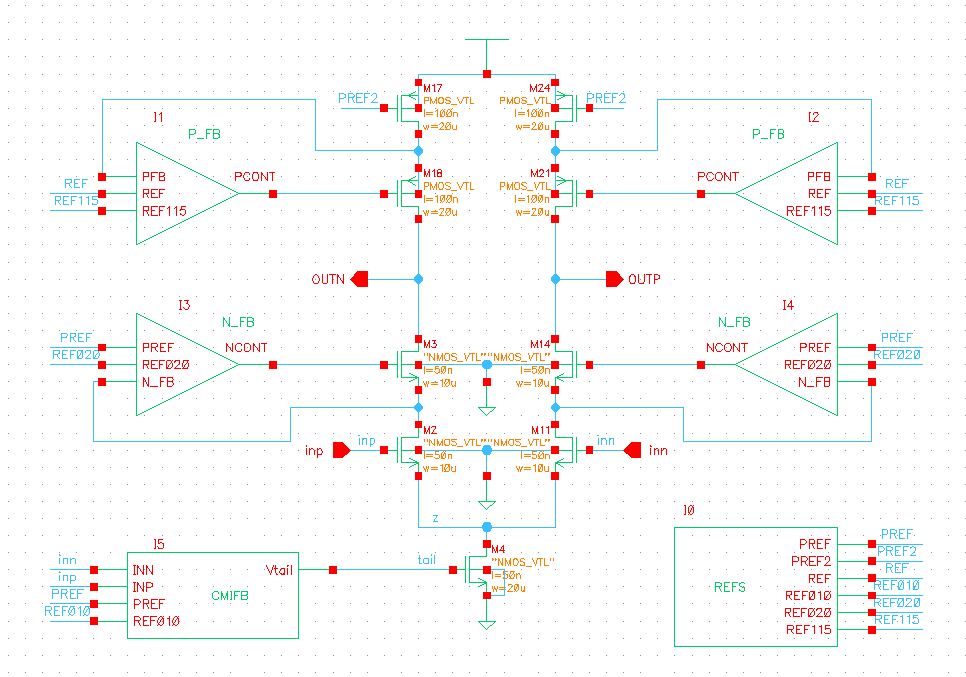
\includegraphics[width=0.5\textwidth]{hierchial_op.png}
\caption{Full Op Amp Schematic}
\label{folded}
\end{figure}
\FloatBarrier

The following is the gain boosting amplifier used on the lower half of the cascode. The design is a two stage op amp with p inputs in order to sense the low 0.1 V signal at the feedback node. This signal is compared to a 0.1V reference in the 5T pair and the output is then buffered through an inverting amplifier. The inv. amplifier output connects to the transistor being controlled by the gain boosting circuit. The sizes for this circuit were selected for 20uA bias and minimal size.
\FloatBarrier
\begin{figure}[htb]
\centering
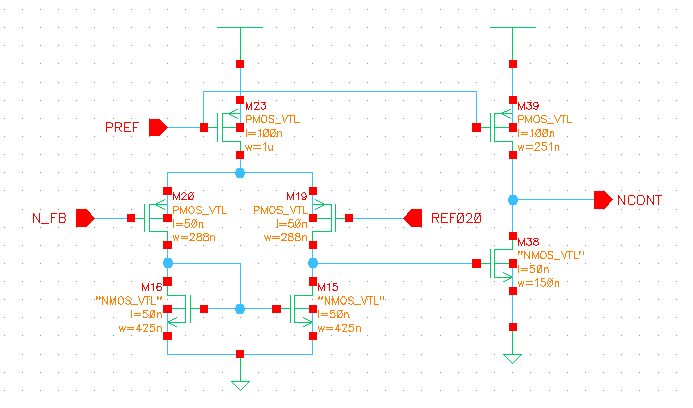
\includegraphics[width=0.5\textwidth]{nfb.png}
\caption{Gain boosting amplifier for the bottom half of the cascode}
\label{folded}
\end{figure}
\FloatBarrier
The next circuit is the gain boosting amp for the P channel device half of the cascode. The operation is the same (complementary) to the previous one so I will not discuss it further. Design considerations were made for 10uA bias currents, minimal channel size, and channel length were found via simulation and selecting the optimal size.

\FloatBarrier
\begin{figure}[htb]
\centering
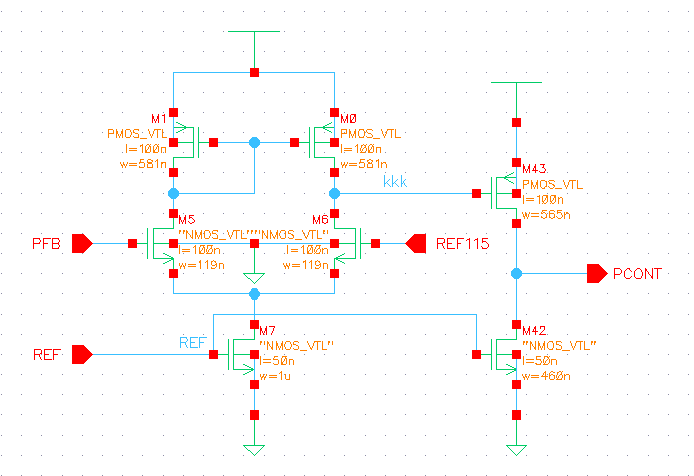
\includegraphics[width=0.5\textwidth]{pfb.png}
\caption{Gain boosting amplifier for the top half of the cascode}
\label{folded}
\end{figure}
\FloatBarrier

The voltage reference for the opamp is shown below. It is implemented using a self-biasing threshold-referenced current referent, which has good supply rejection. This circuit works as the upper half is a current mirror, and the lower is a resistor with a different current transfer reletionship. The circuit operates stably at the intersection of the current transfer curves, with small deviations due to power supply variations. The voltage for the circuit is refered across the resistor as it has the best PSRR. All other bias voltages are generated from this reference voltage using complementry chains of P and NMOS tranistors sized to output the correct voltages when the NMOS is connected to the reference.
\FloatBarrier
\begin{figure}[htb]
\centering
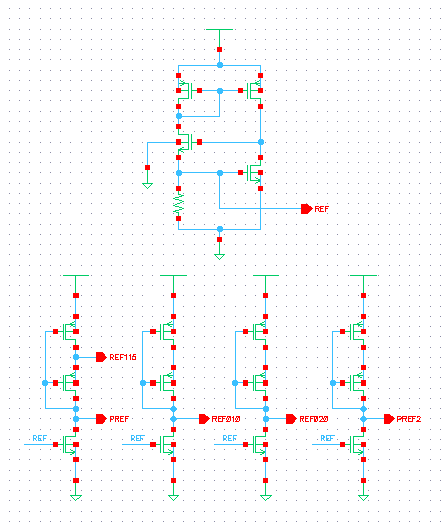
\includegraphics[width=0.5\textwidth]{refs.png}
\caption{Voltage reference generating circuit}
\label{folded}
\end{figure}
\FloatBarrier
The following graphic is a simulation of the voltage out of the reference vs a sweep on supply voltage. We see very little change in the output voltage, approximately a sensitivity of 0.1. This is far lower than what you would see with only using a resistor and a current mirror (0.1) for a reference.

\FloatBarrier
\begin{figure}[htb]
\centering
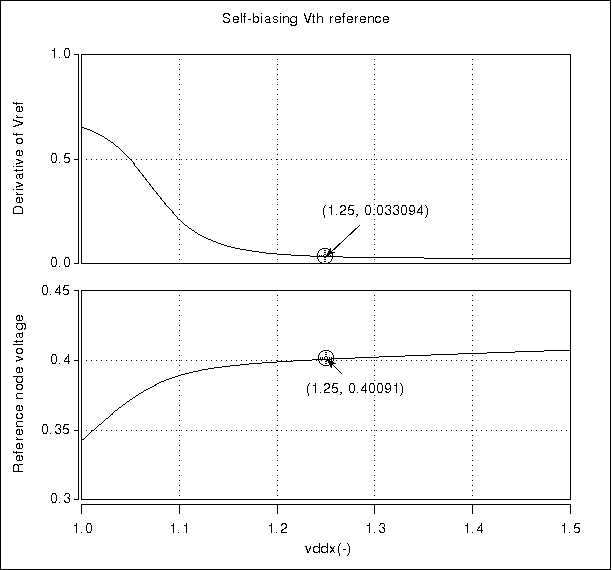
\includegraphics[width=0.5\textwidth]{reference.png}
\caption{Power supply sensitivity of Vth referenced voltage reference}
\label{folded}
\end{figure}
\FloatBarrier

This last circuit is the commom mode feedback circuit for the input. This works by sensing the common mode level with a differential pair connected at both the drain and source, using transistors 1/40 the size of the op amp input transistors, and biased at the same level. THe current from the diff pair is forced through a NMOS 1/40 of the size of the op amp tail transistor, which generates a reference level for the tail transistor that takes in common mode level. An opamp in used to try to force the VDS across the tail transistor to be 0.1 volts at all times to ensure high cascode impedance.
\FloatBarrier
\begin{figure}[htb]
\centering
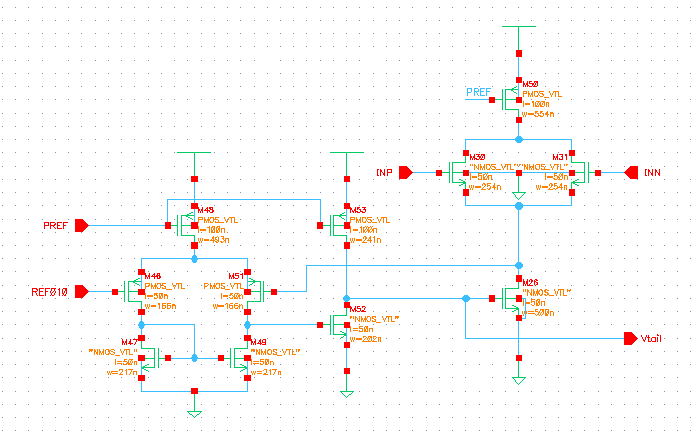
\includegraphics[width=0.5\textwidth]{cmifb.png}
\caption{Input Common mode feedback circuit}
\label{folded}
\end{figure}
\FloatBarrier

The following plot is a VTC for the designed op amp, swept from rail to rail to the input. The outputs cross as intended at half VDD for both output and input. The gain was also extracted by differentiating the curve. The observed gain is 681, or about 56dB, which is quite good. This is nearly 20db better than the design without the gain boosting (gain of 74). Therefore the gain boosting is deemed helpful. Also, the high gain value will help to give a fast rise time, as rise time is at a minimimum 1/GBWP, or 1.37ns.
\FloatBarrier
\begin{figure}[htb]
\centering
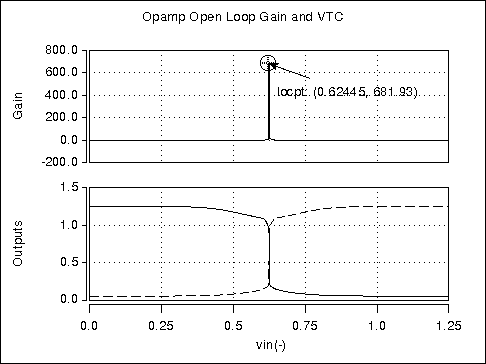
\includegraphics[width=0.5\textwidth]{full_gain_grid.png}
\caption{Op amp VTC with full range sweep and gain extraction}
\label{folded}
\end{figure}
\FloatBarrier
The following is the bode plots for open loop performance of the opamp with 0.5pF of load on each output (1pF total). We see that the unity gain frequency is 731 MHz, with a phase margin of 89 degrees, meaning stablility is given, as well as no ringing.
\FloatBarrier
\begin{figure}[htb]
\centering
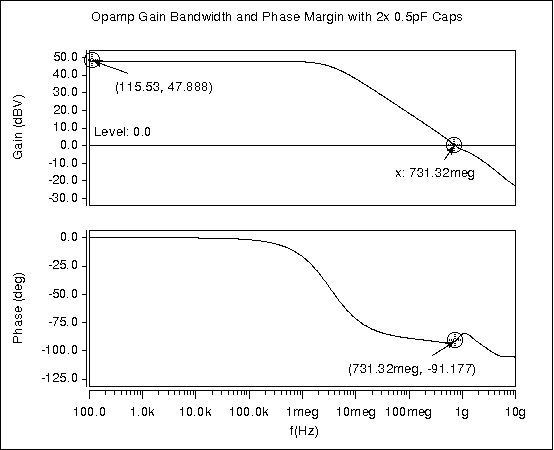
\includegraphics[width=0.5\textwidth]{gbw_pm.png}
\caption{Op Amp Open Loop Bode Plots}
\label{folded}
\end{figure}
\FloatBarrier



\pagebreak
\subsection{OP AMP Layout}
\FloatBarrier
\begin{figure}[htb]
\centering
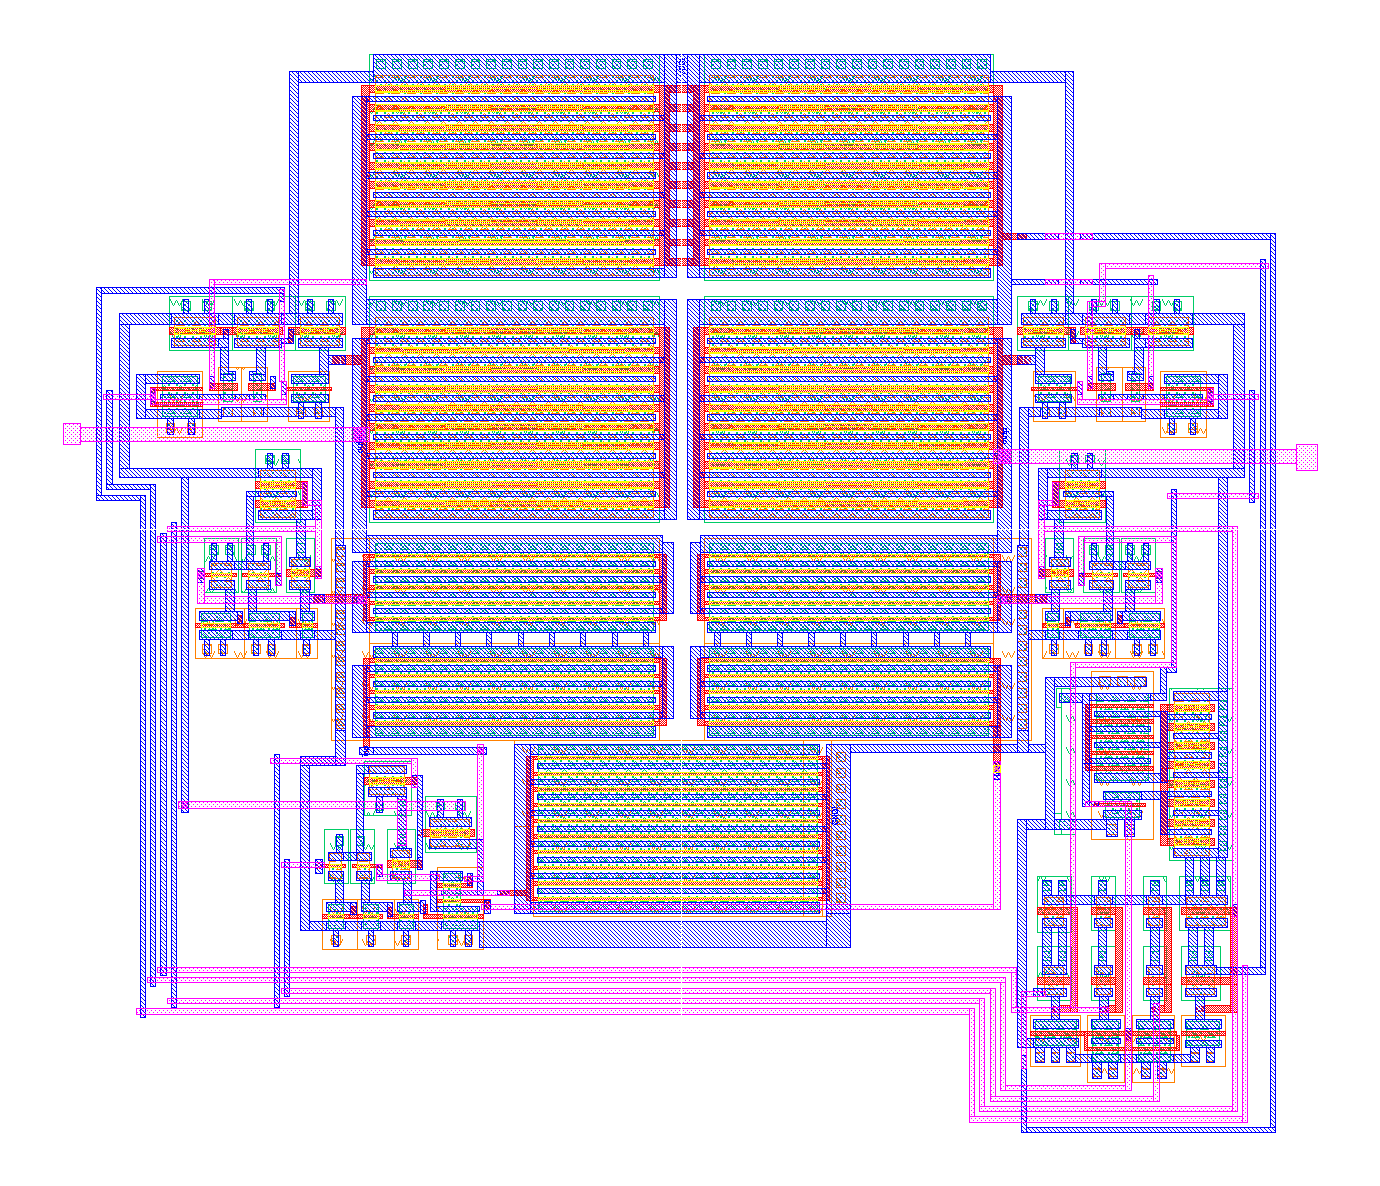
\includegraphics[width=0.5\textwidth]{op_amp_layout.png}
\caption{Layout of the Telescopic Op amp}
\label{folded}
\end{figure}
\FloatBarrier
 The following figure for the design shows the full layout for the opamp. The total size was approximately 17.5 by 15 microns, or 262 sq microns. The center region is the telescopic cascode, the right/left top circuit outside the cascode are the gain boosters, the lower left is the CMFB and the lower right is the ref generator.

\subsection{SC Ciruit}
The circuit designed is duplicated from the first stage of the moving average filter in figure 1's Direct sampling mixer. This is the right half of the schematic below. The left portion is the non-overlapping clock generation circuit, needed to prevent direct feedthrough of signal through the circuit.
\FloatBarrier
\begin{figure}[htb]
\centering
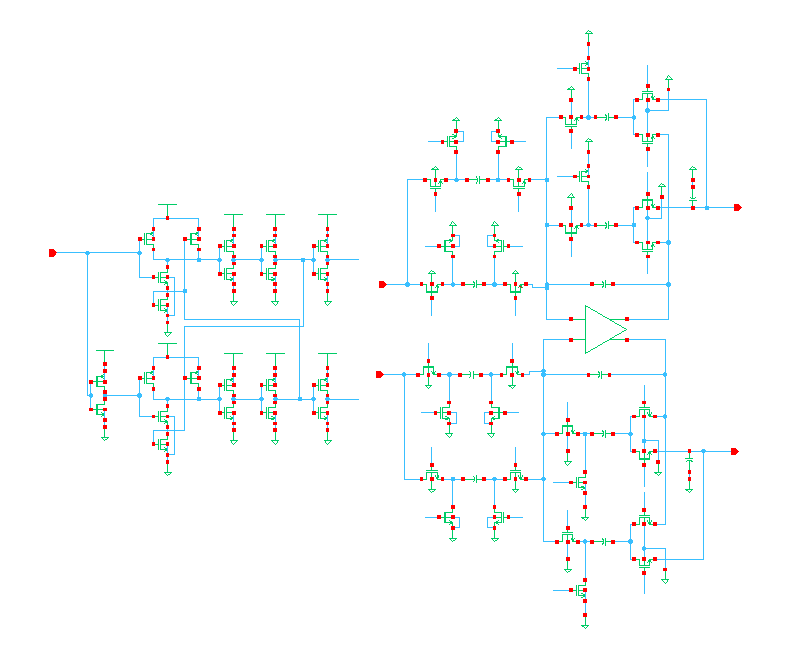
\includegraphics[width=0.5\textwidth]{sc_circuit.png}
\caption{SC Moving Average filter}
\label{folded}
\end{figure}
\FloatBarrier
Below is a gate level schematic of the non-overlapping clock generator. Any clock frequency up to approx 500MHz can be fed in with about 190ps of clock seperation coming out of the two clocks. This circuit was built using standard static CMOS gates.
\FloatBarrier
\begin{figure}[htb]
\centering
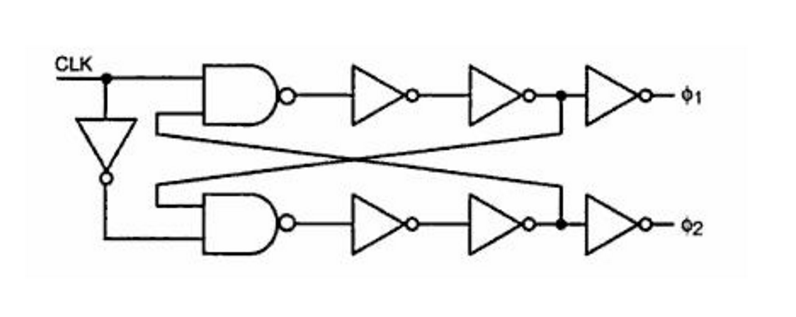
\includegraphics[width=0.5\textwidth]{xxx.png}
\caption{Non-overlapping clock circuit}
\label{folded}
\end{figure}
\FloatBarrier

Below is a plot demonstrating the output of the non-overlapping clock with 200 MHz input. Notice the clock separation.
\FloatBarrier
\begin{figure}[htb]
\centering
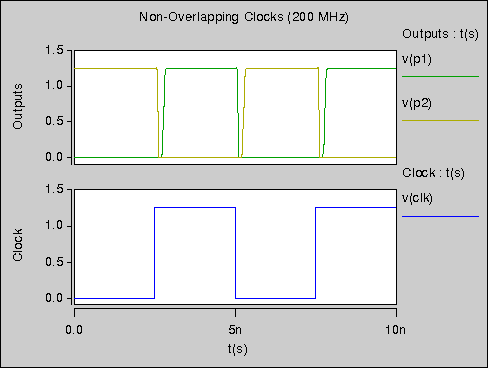
\includegraphics[width=0.5\textwidth]{non_overlap.png}
\caption{Simulation of the non-overlapping clock generator}
\label{folded}
\end{figure}
\FloatBarrier

The following plot is the full layout of the design, having a size of 33 by 16.3 microns. This is about 574 microns squared.


\FloatBarrier
\begin{figure}[htb]
\centering
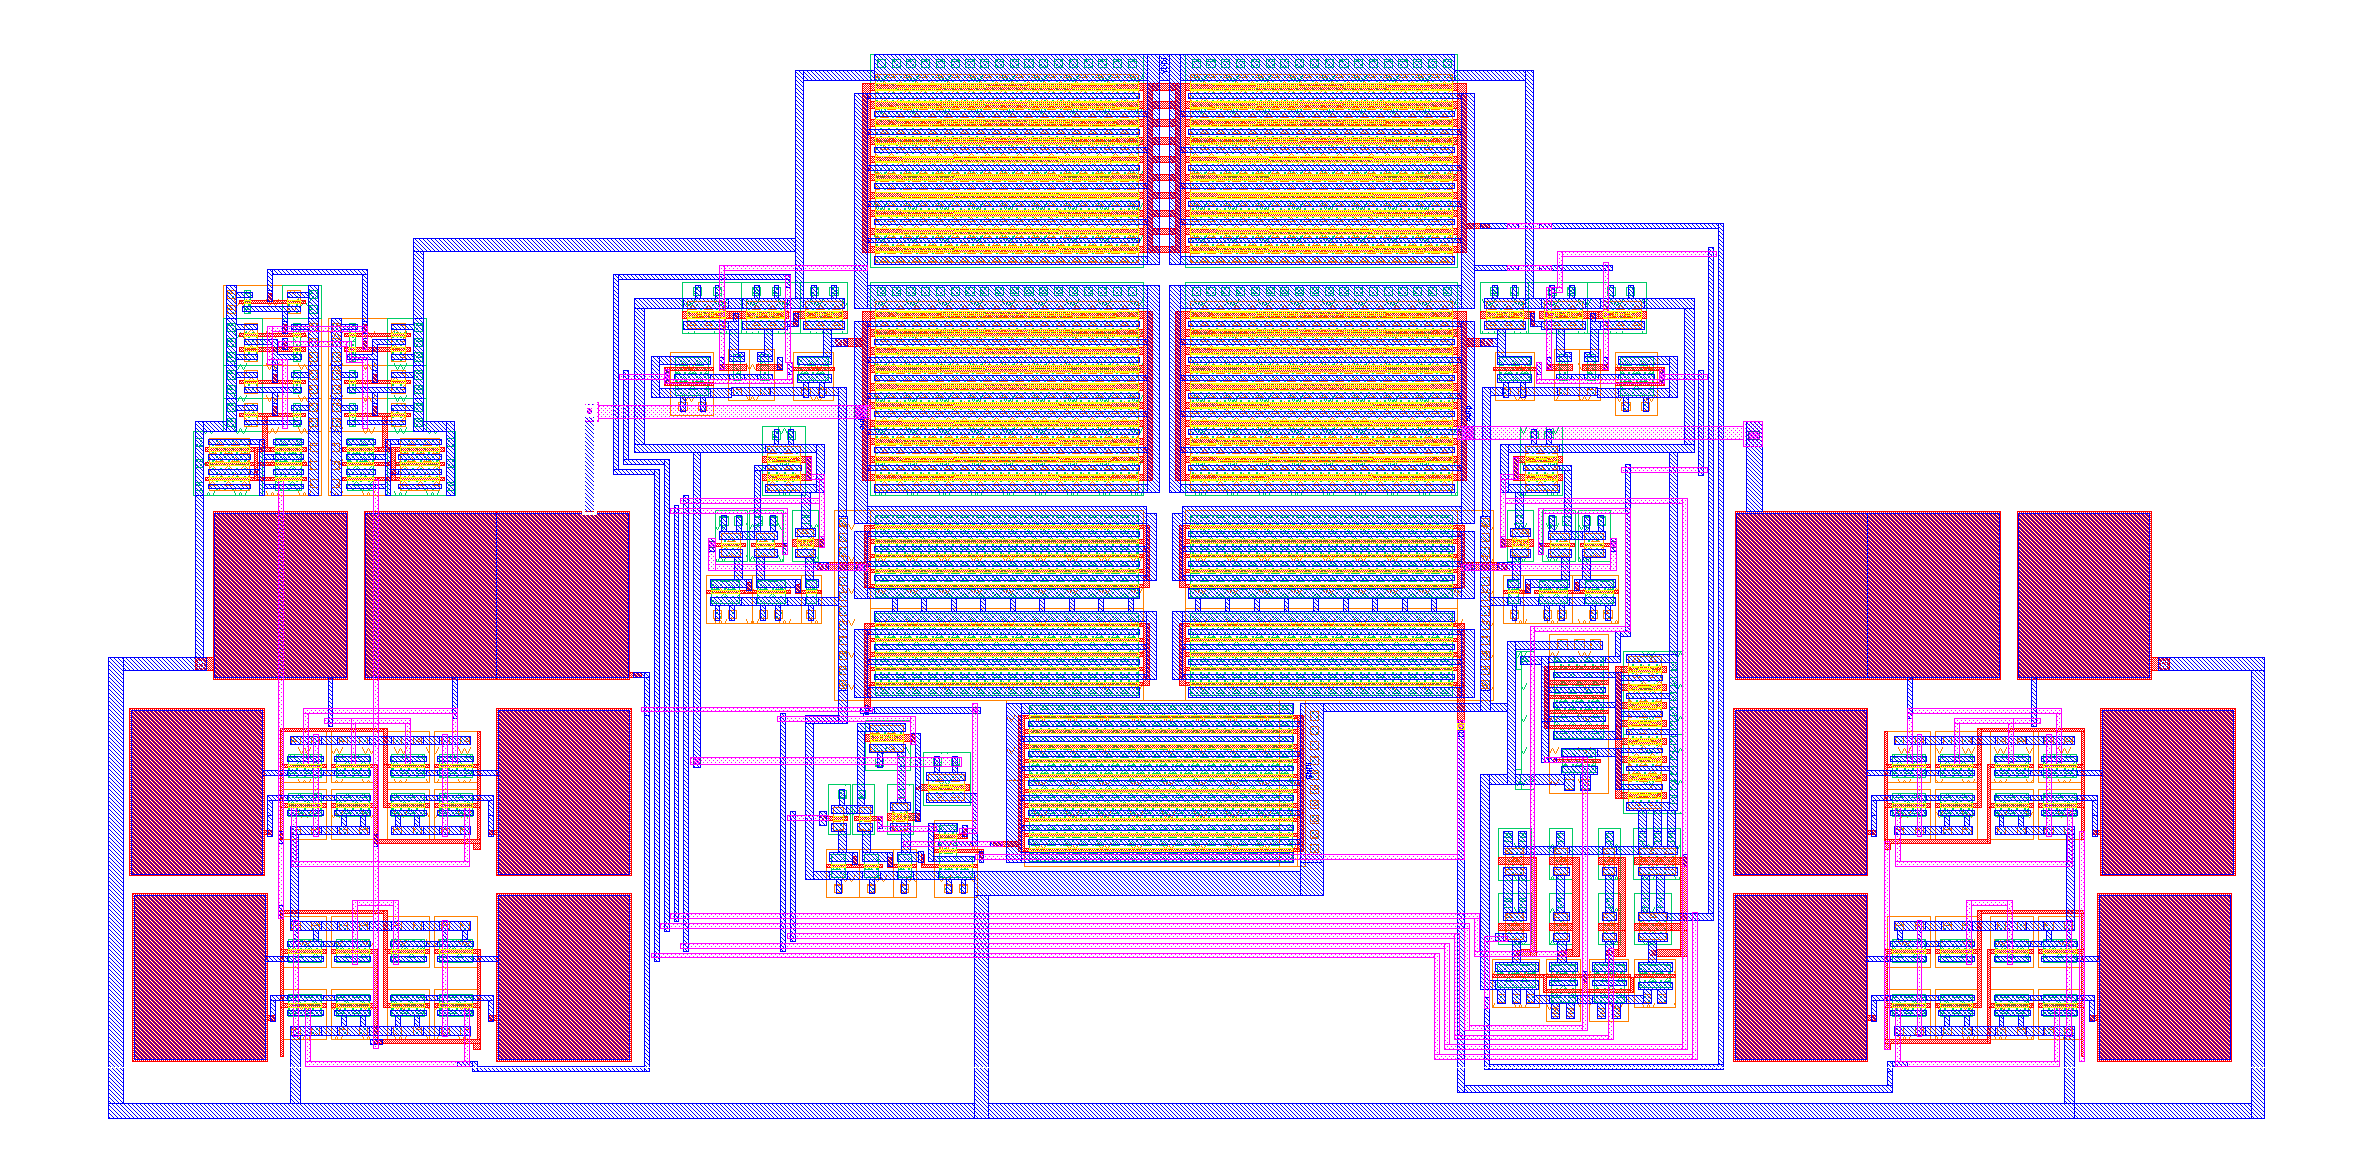
\includegraphics[width=0.5\textwidth]{sc_layout.png}
\caption{Layout of SC circuit}
\label{folded}
\end{figure}
\FloatBarrier
These last two plots show the deficiencies of the opamp in simulation. With a 10MHz signal fed into the amplifier, the output common mode level of the opamp hit the top rail. This was not seen in the OP amp only simulation, so was hard to correct for after designing the op amp. The railing of the output causes the circuit to fail to output any signal (last plot). This would be fixed by implementing better common mode feedback, particularly on the output, however I didn't have time for this.
\FloatBarrier
\begin{figure}[htb]
\centering
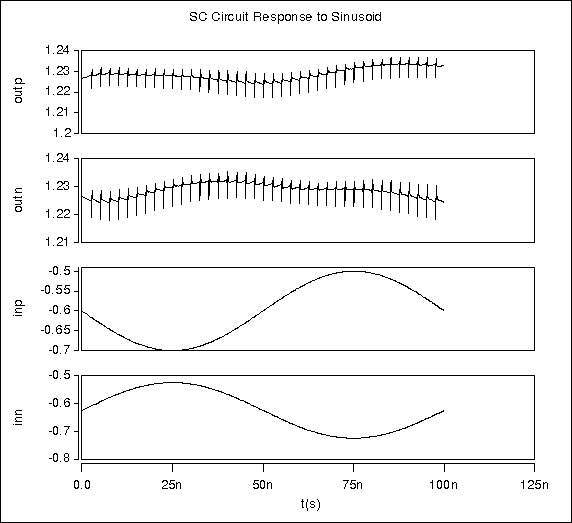
\includegraphics[width=0.5\textwidth]{fgh.png}
\caption{SC circuit simulation output at opamp output nodes}
\label{folded}
\end{figure}
\FloatBarrier

\FloatBarrier
\begin{figure}[htb]
\centering
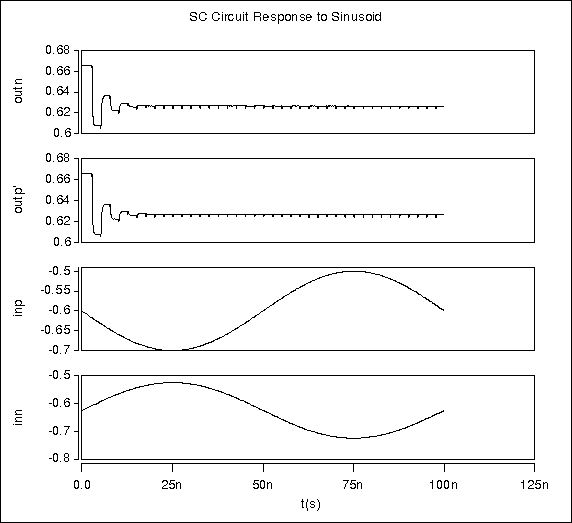
\includegraphics[width=0.5\textwidth]{outputsim.png}
\caption{Time Domain Simulation of SC Circuit}
\label{folded}
\end{figure}
\FloatBarrier








% An example of a floating figure using the graphicx package.
% Note that \label must occur AFTER (or within) \caption.
% For figures, \caption should occur after the \includegraphics.
% Note that IEEEtran v1.7 and later has special internal code that
% is designed to preserve the operation of \label within \caption
% even when the captionsoff option is in effect. However, because
% of issues like this, it may be the safest practice to put all your
% \label just after \caption rather than within \caption{}.
%
% Reminder: the "draftcls" or "draftclsnofoot", not "draft", class
% option should be used if it is desired that the figures are to be
% displayed while in draft mode.
%\includegraphics{universe}
%\begin{figure}[!t]
%\centering
%\includegraphics[width=2.5in]{myfigure}
% where an .eps filename suffix will be assumed under latex, 
% and a .pdf suffix will be assumed for pdflatex; or what has been declared
% via \DeclareGraphicsExtensions.
%\caption{Simulation results for the network.}
%\label{fig_sim}
%\end{figure}

% Note that the IEEE typically puts floats only at the top, even when this
% results in a large percentage of a column being occupied by floats.


% An example of a double column floating figure using two subfigures.
% (The subfig.sty package must be loaded for this to work.)
% The subfigure \label commands are set within each subfloat command,
% and the \label for the overall figure must come after \caption.
% \hfil is used as a separator to get equal spacing.
% Watch out that the combined width of all the subfigures on a 
% line do not exceed the text width or a line break will occur.
%
%\begin{figure*}[!t]
%\centering
%\subfloat[Case I]{\includegraphics[width=2.5in]{box}%
%\label{fig_first_case}}
%\hfil
%\subfloat[Case II]{\includegraphics[width=2.5in]{box}%
%\label{fig_second_case}}
%\caption{Simulation results for the network.}
%\label{fig_sim}
%\end{figure*}
%
% Note that often IEEE papers with subfigures do not employ subfigure
% captions (using the optional argument to \subfloat[]), but instead will
% reference/describe all of them (a), (b), etc., within the main caption.
% Be aware that for subfig.sty to generate the (a), (b), etc., subfigure
% labels, the optional argument to \subfloat must be present. If a
% subcaption is not desired, just leave its contents blank,
% e.g., \subfloat[].


% An example of a floating table. Note that, for IEEE style tables, the
% \caption command should come BEFORE the table and, given that table
% captions serve much like titles, are usually capitalized except for words
% such as a, an, and, as, at, but, by, for, in, nor, of, on, or, the, to
% and up, which are usually not capitalized unless they are the first or
% last word of the caption. Table text will default to \footnotesize as
% the IEEE normally uses this smaller font for tables.
% The \label must come after \caption as always.
%
%\begin{table}[!t]
%% increase table row spacing, adjust to taste
%\renewcommand{\arraystretch}{1.3}
% if using array.sty, it might be a good idea to tweak the value of
% \extrarowheight as needed to properly center the text within the cells
%\caption{An Example of a Table}
%\label{table_example}
%\centering
%% Some packages, such as MDW tools, offer better commands for making tables
%% than the plain LaTeX2e tabular which is used here.
%\begin{tabular}{|c||c|}
%\hline
%One & Two\\
%\hline
%Three & Four\\
%\hline
%\end{tabular}
%\end{table}


% Note that the IEEE does not put floats in the very first column
% - or typically anywhere on the first page for that matter. Also,
% in-text middle ("here") positioning is typically not used, but it
% is allowed and encouraged for Computer Society conferences (but
% not Computer Society journals). Most IEEE journals/conferences use
% top floats exclusively. 
% Note that, LaTeX2e, unlike IEEE journals/conferences, places
% footnotes above bottom floats. This can be corrected via the
% \fnbelowfloat command of the stfloats package.


% conference papers do not normally have an appendix


% use section* for acknowledgment


% trigger a \newpage just before the given reference
% number - used to balance the columns on the last page
% adjust value as needed - may need to be readjusted if
% the document is modified later
%\IEEEtriggeratref{8}
% The "triggered" command can be changed if desired:
%\IEEEtriggercmd{\enlargethispage{-5in}}

% references section

% can use a bibliography generated by BibTeX as a .bbl file
% BibTeX documentation can be easily obtained at:
% http://mirror.ctan.org/biblio/bibtex/contrib/doc/
% The IEEEtran BibTeX style support page is at:
% http://www.michaelshell.org/tex/ieeetran/bibtex/
%\bibliographystyle{IEEEtran}
% argument is your BibTeX string definitions and bibliography database(s)
%\bibliography{IEEEabrv,../bib/paper}
%
% <OR> manually copy in the resultant .bbl file
% set second argument of \begin to the number of references
% (used to reserve space for the reference number labels box)
\begin{thebibliography}{1}

\bibitem{IEEEhowto:allen}
P.~E. Allen and D.~R. Holberg, \emph{CMOS Analog Circuit Design}, 3rd~ed.\hskip 1em plus
  0.5em minus 0.4em\relax Harlow, England: Oxford Univerity Press, 2012.
\bibitem{IEEEhowto:new}
T.~Neu, "Direct RF conversion: From vision to reality," Texas Instruments, Dallas, TX, 2015.
\bibitem{IEEEhowto:razavi}
B.~Razavi, \emph{Analog CMOS Integrated Circuits}, 2nd~ed.\hskip 1em plus
  0.5em minus 0.4em\relax New York, NY: McGraw-Hill Education, 2017.
\bibitem{IEEEhowto:razavi2}
B.~Razavi, \emph{RF Microelectronics}, 1st.~ed.\hskip 1em plus
0.5em minus 0.4em\relax Upper Saddle River, NJ: Prentice Hall, 1998.
\bibitem{IEEEhowto:greg}
R.~Gregorian and G.~C. Temes, \emph{Analog MOS Integrated Circuits for Signal Processing}, 1st~ed.\hskip 1em plus
  0.5em minus 0.4em\relax Wiley, 1986.
\bibitem{IEEEhowto:stas}
R. B.~Staszewski, et al., "All-Digital TX Frequency Synthesizer and Discrete-Time Receiver for Bluetooth Radio in 130-nm CMOS", \emph{IEEE Journal of Solid-State Circuits Conf.,} Vol. 39, No. 12, pp. 2278-2291, Dec. 2004.
\bibitem{IEEEhowto:ninh}
H. P.~Ninh, T.~Moue, T.~Kurashina, K.~Okada and A.~Matsuzawa, "A CMOS Direct Sampling Mixer
Using Switched Capacitor Filter Technique for Software-Defined Radio", \emph{Asia and South Pacific Design Automation Conference}, Mar. 2008.
\bibitem{IEEEhowto:jian}
X.~Jiangtao, Carlos E.~Saavedra and C.~Guican, "A CMOS wideband front-end chip using direct RF sampling mixer with embedded discrete-time filtering", \emph{Chinese Institute of Electronics Journal of Semiconductors}, Vol. 32, No. 8, 2011.
\end{thebibliography}




% that's all folks
\end{document}


